\documentclass[12pt]{article}
% load the necessary packages
\usepackage[paperheight=1in,paperwidth=18in,margin=0in]{geometry}
\usepackage{pdftricks}
\begin{psinputs}
  \usepackage[dvipsnames,prologue,table]{pstricks}
	\usepackage{pst-text}
	\usepackage{pst-char}
	\usepackage{pst-grad}
	\psset{unit=1in}
\end{psinputs}
\usepackage{graphicx}
\usepackage{lipsum}
% begin the document and suppress page numbers

\begin{document}
\pagestyle{empty}
% create the box with the front cover picture
\newsavebox\IBox
\sbox\IBox{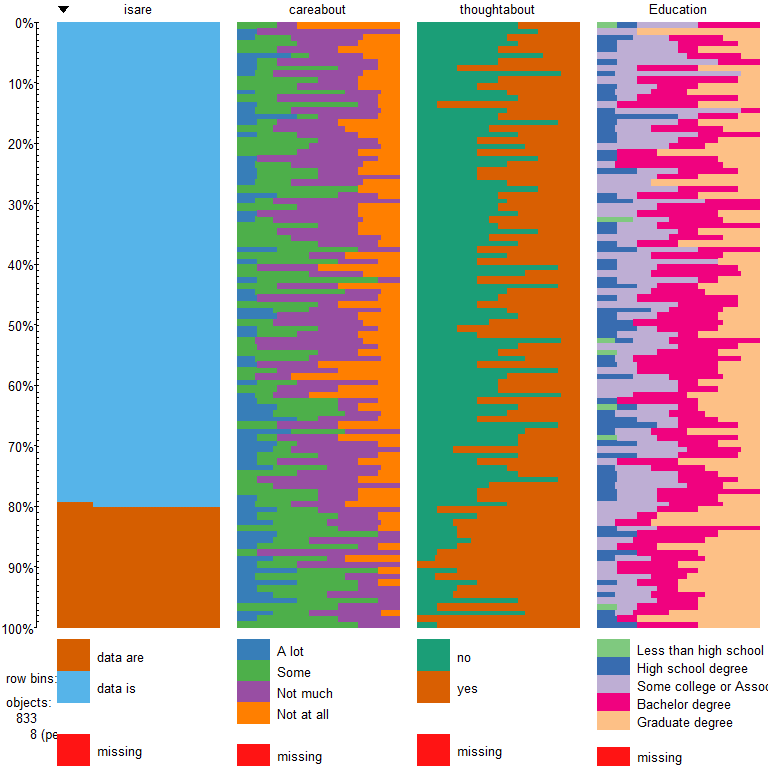
\includegraphics[height=6in]{cover_image_v3.png}}
% set up the picture environment

\begin{pdfpic}
\begin{pspicture}(18in,11in)
% set up the fonts we use
\DeclareFixedFont{\PT}{T1}{ppl}{b}{it}{0.5in}
\DeclareFixedFont{\PTsmall}{T1}{ppl}{b}{it}{0.4in}
\DeclareFixedFont{\PTsmallest}{T1}{ppl}{b}{it}{0.3in}
\DeclareFixedFont{\PTtext}{T1}{ppl}{b}{it}{11pt}
\DeclareFixedFont{\Logo}{T1}{pbk}{m}{n}{0.3in}
% create a maroon background
\psframe[fillstyle=solid,fillcolor=White](0,0)(18,11)
23
% place the front cover picture
\rput[lb](10.5,0){\usebox\IBox}
% put the text on the front cover
\rput[lb](10.5,9.75){\PT \color{Orange}{A Second Semester Statistics}}
\rput[lb](11.75,9){\PT \color{Orange}{Course with R}}
\rput[lb](11.25,8.25){\PTsmall\color{black}{Mark Greenwood and Katharine Banner}}
\rput[lb](12.75,8){\PTsmall\color{black}{\itshape {Version 4.0}}}
\rput[lb](12.25,7.5){\PTsmall\color{black}{Published Fall 2017}}
% put the text on the spine (note the rotation over 270 degrees)
\rput[l]{270}(6.62,8.5){\PTsmall%
\color{black}{Greenwood and Banner\hspace{0.25in}2017\hspace{0.25}A Second Semester Statistics Course with R}}
\end{pspicture}
\end{pdfpic}
\end{document}